\section{Exact Local Demand Calculus}
\label{sec:exact-local-demand-calculus}

This section develops the local calculus for configurations in which a coarse
length sum does not by itself record enough information.  The mechanism is
always the same.  A center trace fixes boundary inputs and complementary
radial demands; an exact
local map propagates these data through nonsupercritical rows; and the
returning demand exceeds the remaining boundary or radial capacity.

Actual maximal reaches continue to be denoted by $(A_i,B_i,C_i)$, while
lowercase letters denote prescribed demands.  Every estimate in this section
is proved analytically.  In particular, no empirical branch catalogue,
machine-assisted certificate, or formal root from a discarded algebraic
component is used.

\subsection{The exact local feasible set}

Put
\[
 u=\left(\frac12,\frac{\sqrt3}{2}\right),\qquad
 v=\left(\frac12,-\frac{\sqrt3}{2}\right).
\]
For $0\le a,b,c\le1$ define
\[
 K(a,b,c)=\conv\{0,au,bv,c(u+v)\}.
\]
Thus $a,b$ are lower demands on the two incident boundary rays and $c$ is a
lower demand on the inward radial ray.

\begin{definition}
\label{def:admissible-demands}
The local admissible set is
\[
 \begin{aligned}
 \mathcal A=\{(a,b,c)\in[0,1]^3:\;&K(a,b,c)\text{ is contained}\\
 &\text{in a closed unit equilateral triangle}\}.
 \end{aligned}
\]
For $a,c\in[0,1]$ put
\[
 \begin{aligned}
 B_c(a)&=\max\{b:(a,b,c)\in\mathcal A\},\\
 F_c(a)&=\min\{B_c(a),1-a\},\\
 G_c(a)&=1-F_c(a).
 \end{aligned}
\]
\end{definition}

The distinction between demands and actual reaches is important.  If a role
has actual reaches $(A,B,C)$ and $A\ge a$, $C\ge c$, then $(a,B,c)$ is a
demand triple realized by the same role.  If in addition $A+B\le1$, then
\begin{equation}
 B\le F_c(a).
 \label{eq:safe-capped-bound}
\end{equation}
No assertion about the type of a maximizing triangle is required.

\begin{proposition}[Exact admissible set and radial envelope]
\label{prop:exact-admissible-set}
\label{prop:local-admissible}
Put
\[
 s=a+b,\qquad d=a^2+ab+b^2,\qquad
 m=\min\{a,b\},\qquad M=\max\{a,b\},
\]
and
\[
 q=s^4-s^2+ab.
\]
Define
\begin{align*}
 F_L(a,b,c)&=c^4-c^2+mc-m^2,\\
 F_T(a,b,c)&=(s^2-1)c^2+Mc-M^2,\\
 F_S(a,b,c)&=(m^2-1)c^2+(2mM^2+M)c+M^4-M^2.
\end{align*}
Then $\mathcal A=\mathcal A_L\cup\mathcal A_T\cup\mathcal A_S$, where
\begin{align*}
 \mathcal A_L&=\{d\le1, s\le1, q\le0, F_L\le0\},\\
 \mathcal A_T&=\{d\le1, s\le1, q\ge0, F_T\le0, c\le2M\},\\
 \mathcal A_S&=\{d\le1, s>1, F_S\le0, c\le\tfrac12\}.
\end{align*}
All variables in these three sets are also constrained to $[0,1]$.

For $d\le1$, the maximal radial demand is
\begin{equation}
 c_{\max}(a,b)=
 \begin{cases}
  1,&a=b=0,\\
  C_L(m),&s\le1, q\le0, (a,b)\ne(0,0),\\
  C_T(m,M),&s\le1, q>0,\\
  C_S(m,M),&s>1,
 \end{cases}
 \label{eq:radial-envelope}
\end{equation}
where $C_L(m)$ is the unique root in $[\sqrt3/2,1]$ of
\[
 z^4-z^2+mz-m^2=0,
\]
and
\[
 C_T(m,M)=\frac{2M}{1+\sqrt{4s^2-3}},
\qquad
 C_S(m,M)=
 \frac{M(2mM+1)-M\sqrt{4d-3}}{2(1-m^2)}.
\]
If $d>1$, the radial envelope is undefined.  At $q=0$ the two subcritical
formulas agree and equal $s$.
\end{proposition}

\begin{proof}
If $s>0$ and $cs\le ab$, then $c/a+c/b\le1$ (with the zero-coordinate
cases obtained by continuity), so $c(u+v)$ lies in
$\conv\{0,au,bv\}$.  Its minimum enclosing equilateral side is the diameter
\[
 \sqrt{a^2+ab+b^2}.
\]
Assume now that $cs>ab$.  The four points occur cyclically as
$0,bv,c(u+v),au$.  For three outward unit normals separated by
$120^\circ$, the required side equals $2/\sqrt3$ times the sum of the three
support values.  On an angular cell with fixed support points this sum has
second derivative equal to its negative.  Hence an angular minimum occurs
when a normal is perpendicular to one of the four hull edges.  The four
resulting side lengths are
\begin{align*}
 L_{0A}&=b+\max\{a,c\},&
 L_{B0}&=a+\max\{b,c\},\\
 L_{AC}&=
 \begin{cases}
 (a^2+bc)/\sqrt{a^2-ac+c^2},&a\ge c,\\
 c(a+b)/\sqrt{a^2-ac+c^2},&a<c\le a+b,\\
 c^2/\sqrt{a^2-ac+c^2},&c>a+b,
 \end{cases}
\end{align*}
and $L_{CB}$ is obtained by interchanging $a,b$.  Thus the minimum side is
the minimum of these four expressions.

Ordering $a,b$ as $m\le M$, squaring the positive support equations gives
$F_L=0,F_T=0,F_S=0$ in the three respective contact regimes; the inactive
support inequalities give $q\le0,q\ge0,s>1$.  Squaring creates one spurious
component in each of the last two cells.  In the $T$ cell the two roots are
\[
 \frac{2M}{1+\sqrt{4s^2-3}},
 \qquad
 \frac{2M}{1-\sqrt{4s^2-3}},
\]
and $c\le2M$ selects the first.  In the $S$ cell the smaller root lies below
$1/2$ and the other above $1/2$; hence $c\le1/2$ is exactly the geometric
selector.  The $L$ fiber is the interval from zero to its unique selected
root.  Solving the selected equations gives \eqref{eq:radial-envelope}.
This also proves that $\mathcal A$ is coordinatewise down-closed.
\end{proof}

\subsection{The exact capped map}

For $1/2<c<1$ put
\[
 \ell(c)=\frac c2\left(1-\sqrt{4c^2-3}\right),\qquad
 r(c)=c-\ell(c)
\]
when $c\ge\sqrt3/2$, and
use the order-transition function $h(c)$ from
\eqref{eq:signed-order-transition}.
Also define
\begin{align*}
 T_-(a,c)&=\frac{\sqrt{a^2-ac+c^2}}c-a,\\
 T_+(a,c)&=
 \frac{2(1-a^2)c^2}
 {2ac^2+c+\sqrt{(2ac^2+c)^2-4(1-c^2)(1-a^2)c^2}}.
\end{align*}

\begin{proposition}[Four-label capped map]
\label{prop:capped-demand-map}
For $1/2<c\le\sqrt3/2$,
\begin{equation}
 F_c(a)=
 \begin{cases}
  1-a,&0\le a\le1-c,\\
  T_+(a,c),&1-c<a<h(c),\\
  h(c),&a=h(c),\\
  T_-(a,c),&h(c)<a<c,\\
  1-a,&c\le a\le1.
 \end{cases}
 \label{eq:S2-capped-map-low}
\end{equation}
For $\sqrt3/2<c<1$,
\begin{equation}
 F_c(a)=
 \begin{cases}
  1-a,&0\le a\le1-c,\\
  T_+(a,c),&1-c<a\le\ell(c),\\
  \ell(c),&\ell(c)<a<r(c),\\
  T_-(a,c),&r(c)\le a<c,\\
  1-a,&c\le a\le1.
 \end{cases}
 \label{eq:S2-capped-map-high}
\end{equation}
Thus there are exactly four labels
\[
 \mathrm{Full},\qquad L,\qquad T_-,\qquad T_+^{\mathrm{hi}}.
\]
At $a=\ell(c)$ in \eqref{eq:S2-capped-map-high},
$F_c(a)=r(c)$; immediately to its right the value is $\ell(c)$.  This
downward jump is genuine.  The formal other root of the $T_+$ quadratic is
not feasible because it violates $c\le2\max\{a,F_c(a)\}$.

The maps $F_c$ are nonincreasing, the maps $G_c=1-F_c$ are nondecreasing
and extensive, and
\begin{equation}
 G_c(a)\le z\quad\Longleftrightarrow\quad
 G_c(1-z)\le1-a.
 \label{eq:S2-capped-duality}
\end{equation}
\end{proposition}

\begin{proof}
The cap $a+b\le1$ eliminates the $S$ cell of
Proposition~\ref{prop:exact-admissible-set}.  On the cap $b=1-a$, the $T$
inequality reduces to $M(c-M)\le0$; hence the Full face is feasible exactly
for $a\le1-c$ or $a\ge c$.  Off that face a maximal point lies on $F_L=0$
or $F_T=0$.  The $L$ equation has roots $\ell(c),r(c)$ and the selector
$q\le0$ keeps only the smaller coordinate.  The ordered $T$ halves give
respectively the displayed lower quadratic root $T_+$ and the root $T_-$.
Their order boundary is $a=b=h(c)$, while their $q=0$ boundaries are
$(\ell(c),r(c))$ and $(r(c),\ell(c))$.  These observations give
\eqref{eq:S2-capped-map-low}--\eqref{eq:S2-capped-map-high}, including all equality
assignments.

Down-closedness gives monotonicity, while $F_c(a)\le1-a$ gives
$G_c(a)\ge a$.  Finally,
\[
 G_c(a)\le z\iff F_c(a)\ge1-z
 \iff(a,1-z,c)\in\mathcal A,\quad a+1-z\le1.
\]
Reflection $a\leftrightarrow b$ gives \eqref{eq:S2-capped-duality}.
\end{proof}

Put
\[
 \mu=\frac{2\sqrt3-3}{4},
\]
and, for $0<X<1-\sqrt3/2$, write
\[
 e(X)=\ell(1-X).
\]
The root equation gives
\begin{equation}
 \begin{aligned}
 X&<e(X) &&\left(0<X<1-\frac{\sqrt3}{2}\right),\\
 e(X)&<\frac{2X}{1-2X} &&(0<X\le\mu),\\
 e(X)&\le2X+5X^2 &&(0<X\le1/8).
 \end{aligned}
 \label{eq:low-root-bounds}
\end{equation}
Moreover,
\begin{equation}
 a>e(X)\quad\Longrightarrow\quad
 G_{1-X}(a)\ge1-e(X)
 \qquad\left(0<X<1-\frac{\sqrt3}{2}\right).
 \label{eq:high-demand-threshold}
\end{equation}
Indeed, for
\[
 p_X(z)=z^2-(1-X)z+(1-X)^2-(1-X)^4,
\]
one has
\[
 p_X(X)=X(1-3X+4X^2-X^3)>0.
\]
Since $X<(1-X)/2$, this puts $X$ strictly below the smaller root $e(X)$.
For $U=2X/(1-2X)$, direct substitution gives
\[
 p_X(U)=-\frac{X^2}{(1-2X)^2}
 (4X^4-20X^3+37X^2-28X+3).
\]
The polynomial in parentheses is decreasing on $[0,\mu]$ and at the right
endpoint equals $8217/64-74\sqrt3>0$.  Indeed, its derivative is at most
$16/512+74/8-28<0$, and
$(8217/64)^2-3\mathbin{\cdot}74^2=230001/4096>0$.  Hence $p_X(U)<0$, which puts $U$
strictly between the roots.  Finally,
\[
 p_X(2X+5X^2)=X^2(3X+4)(8X-1)\le0,
\]
and $X<2X+5X^2<(1-X)/2$ on the stated range.  Thus the trial point lies
between the two roots, proving the third comparison.  The implication
\eqref{eq:high-demand-threshold} is read directly from
\eqref{eq:S2-capped-map-high}.  We shall also use
$e(X)<2X+3X^2$ for $0<X\le1/10$, obtained from
$p_X(2X+3X^2)=X^2(8X^2+19X-2)<0$; here too the trial point lies strictly
between $X$ and $(1-X)/2$.

\section{Cyclic Propagation in the All-$\Vdzero$ Cases}
\label{sec:cyclic-all-vd0}

\subsection{The exactly-one-supercritical all-$\Vdzero$ branch}

For a center interval, call the nonempty closed set missed by its two open
endpoint roles a \emph{V-gap}.  It may be a singleton.  If the maximal
closed center trace is $[s,t]$, open coverage gives the weak bounds
$B_i\ge s$ and $A_{i+1}\ge1-t$; thus none of the arguments below discards a
singleton gap.

\begin{proposition}[CE1 one-gap five-map obstruction]
\label{prop:ce1-one-gap}
Assume that every vertex role is $\Vdzero$, $N_+=1$, and the center role is
CE1.  If its boundary trace contains a V-gap, the roles do not cover $H$.
\end{proposition}

\begin{proof}
Use the signed center variables of
Proposition~\ref{prop:signed-center-normal-form}, and put
\[
 w=W,\qquad A=\alpha,\qquad D=\delta,\qquad
 X=R-D,\qquad H=\frac{\eta+A+D}{2R}.
\]
The CE1 sign gives
$D+RA\ge P$ and $RD>wA$, so
\[
 m_3=\min\left\{\frac AR,\frac Dw\right\}=\frac AR.
\]
The exact strict domain needed below is
\begin{equation}
\begin{gathered}
 A>0,\quad D>0,\quad A+wD<P,\quad D+RA\ge P,\\
 A<\frac w2,\quad D<\frac R2,\quad RD-wA>0,
\end{gathered}
\label{eq:ce1-normal-domain}
\end{equation}
Proposition~\ref{prop:signed-one-gap-interface} contains the five actual-row
handoffs, the three duality steps, and the terminal diameter comparison.
It remains only to prove its scalar target
\begin{equation}
 \left(G_{1-D}\circ G_{1-m_3}\circ G_{1-A}\right)(H)>1-X.
 \label{eq:ce1-suffix}
\end{equation}
Here $A<P\le\mu$, because $P=E(1-E)$ and $E\ge\sqrt3/2$.  We first prove
the two input comparisons used at row $4$.  Since $D=R-X$, the inequality
$A+wD<P$ and the identity $Rw=\eta+P$ give
\[
 A<wX-\eta.
\]
Put
\[
 \varphi(q)=wq-\frac{q}{2(1+q)}.
\]
The bound $0<D<R/2$ gives $R/2<X<R$, and $\varphi$ is convex.  At the
endpoints,
\[
 \varphi(R/2)<\frac{Rw}{2}<\eta,
\]
while $\varphi(R)<\eta$ is equivalent to
\[
 E(1-2R^2)<1,
\]
which follows from $E<1$.  Convexity therefore gives
$\varphi(X)<\eta$, and hence
\[
 A<\frac{X}{2(1+X)}.
\]
Using the rational low-root bound in its valid range,
\begin{equation}
 e(A)<\frac{2A}{1-2A}<X.
 \label{eq:ce1-first-low-root}
\end{equation}
We also have
\[
 2R(H-A)=\eta+D+(1-2R)A.
\]
This is positive if $R\le1/2$.  If $R>1/2$, then $A<P=\eta E$ gives
\[
 2R(H-A)>
 \eta\bigl(1-(2R-1)E\bigr)>0.
\]
Thus $H>A$.  The positive signed right trace gives
\[
 \frac{\eta+A+D}{R}<w+D<1,
\]
so $H<1/2<1-A$.

Now consult the exact high-radial catalog for $c_4=1-A$.  The lower and
upper Full ranges would require $H\le A$ and $H\ge1-A$, respectively, so
both are impossible.  On the $L$ or $T_-$ range,
\[
 F_{1-A}(H)\le e(A),
\]
and therefore
\[
 G_{1-A}(H)\ge1-e(A)>1-X
\]
by \eqref{eq:ce1-first-low-root}.  Thus only the
$T_+^{\rm hi}$ range remains.  Its selector gives
\[
 H\le e(A)\le2A+5A^2.
\]
We claim that this range forces $X>1/2$.  Indeed, if $X\le1/2$, the selector
and the lower center inequality give
\[
 2RH=\eta+A+D\ge\eta+P+wA=w(R+A).
\]
Together with $H<2A/(1-2A)$, this implies
\[
 f_R(A)<0,
 \qquad
 f_R(z):=w(R+z)(1-2z)-4Rz.
\]
But $f_R''(z)=-4w<0$ and $f_R(0)=Rw>0$.  We check the other endpoint of
the possible interval for $A$.

If $R\le1/2$, then $0<A<P$.  Direct simplification gives
\[
 f_R(P)
 =(1-E)\left(
 4E^3-2E^2+1-R(2E^3-2E^2+5E)
 \right).
\]
The coefficient of $R$ is positive, so
\[
 f_R(P)\ge
 \frac{1-E}{2}\left(6E^3-2E^2-5E+2\right).
\]
For $\phi(E)=6E^3-2E^2-5E+2$ on
$[\sqrt3/2,1)$,
\[
 \phi'(E)=18E^2-4E-5
 \ge\frac{17}{2}-2\sqrt3>0,
\]
and
\[
 \phi\left(\frac{\sqrt3}{2}\right)
 =\frac{2-\sqrt3}{4}>0.
\]
Hence $f_R(P)>0$.  Strict concavity puts $f_R$ above its endpoint chord,
so $f_R(A)>0$ for $0<A<P$, a contradiction.

If $R>1/2$, the assumption $X\le1/2$ gives
$D\ge R-1/2$, and therefore
\[
 0<A<A_0,
 \qquad
 A_0:=P-w\left(R-\frac12\right)=\frac w2-\eta.
\]
Direct simplification gives
\[
 f_R(A_0)
 =\frac{1-E}{2}(E+11R-3ER-5).
\]
Since $11-3E>0$ and $R>1/2$,
\[
 E+11R-3ER-5
 >\frac{11-3E}{2}+E-5
 =\frac{1-E}{2}>0.
\]
Thus $f_R(A_0)>0$.  Concavity again gives $f_R(A)>0$ on $(0,A_0)$, a
contradiction.  Both ranges are impossible, proving $X>1/2$.

Put $p_1=G_{1-A}(H)$.  If row $3$ is not $T_+^{\rm hi}$, then
$p_1\le A+e(A)<3A+5A^2<29/64<1/2$, and
$2R(H-m_3)=\eta+D-A>\eta-P>0$.  Extensivity gives
$p_1\ge H>m_3$, while $p_1<1/2<1-m_3$; thus both Full ranges are impossible.
On $L$, $T_-$, or the low-$c$ tie one has $F_{1-m_3}(p_1)\le p_1$, so
\[
 G_{1-m_3}(p_1)\ge1-p_1>1-X.
\]
Extensivity of the final reverse map $G_{1-D}$ preserves this strict bound
and proves \eqref{eq:ce1-suffix}.  It remains to treat the selected row-$3$
$T_+$ branch.  Proposition~\ref{prop:reader-universal-tplus} proves once
for all that every selected $T_+$ arc is increasing and strictly concave.

When $d<1-\sqrt3/2$, the arc endpoints are
$(d,d)$ and $(e(d),d+e(d))$, so concavity gives
\begin{equation}
 q\ge p+\frac{d}{e(d)-d}(p-d).
 \label{eq:ce1-selected-chord}
\end{equation}
For $0<d\le\mu$, the valid rational low-root bound gives
\[
 \frac{d}{e(d)-d}>\frac{1-2d}{1+2d}>1-4d>1-5d.
\]
This covers row $4$, because its parameter is $d=A<P\le\mu$.  For the
row-$3$ parameter $d=m_3$, which need not be at most $\mu$, the remaining
high-radial range is handled without the rational estimate.  If
$\mu<d\le1/8$, then
\[
 \frac{d}{e(d)-d}\ge\frac1{1+5d}>1-5d
\]
by $e(d)\le2d+5d^2$.  If
$1/8<d<1-\sqrt3/2$, then $e(d)<(1-d)/2$ and hence
\[
 \frac{d}{e(d)-d}>\frac{2d}{1-3d}>1-5d.
\]
The last comparison is equivalent to $15d^2-10d+1<0$; its smaller root
$(5-\sqrt{10})/15$ is less than $1/8$.  In the low-$c$ row-$3$ range
$1-\sqrt3/2\le d<1/5$, the other endpoint is
$(h(1-d),1-h(1-d))$, and the chord coefficient is
\[
 \frac{1-2h(1-d)}{h(1-d)-d}.
\]
On $3/4\le c\le\sqrt3/2$, direct differentiation of the formula for $h$
shows that $h(c)$ is nonincreasing.  Moreover,
\[
 h\left(\frac34\right)
 =\frac{3}{2(\sqrt6+1)}<\frac7{16}.
\]
Here low $c$ gives $d\ge1-\sqrt3/2>2/15>1/16$, and hence
\[
 h(1-d)<\frac7{16}<\frac{3+d}{7}.
\]
Thus the displayed chord coefficient is greater than $1/3$, while
$1-5d<1/3$.
For $d\ge1/5$, extensivity alone is stronger than the row-$3$ estimate.

Applying these chord bounds first with $d=A$ and then with $d=m_3$ proves,
without an omitted selected branch,
\begin{align*}
 p_1&>L_1:=(2-4A)H-(1-4A)A,\\
 p_2:=G_{1-m_3}(p_1)&>L_2:=(2-5m_3)L_1-(1-5m_3)m_3.
\end{align*}

Finally let
\[
 D_0=P-RA,\qquad
 D_h=A(4R-1)+10RA^2-\eta,\qquad x=Rw.
\]
Feasibility puts $D_0\le D\le D_h$.  We first prove that the actual
feasible value satisfies $D<1/10$.  Since
\[
 P=\frac{xE}{1+E}<\frac x2,\qquad
 \eta=\frac{x}{1+E}>\frac x2,
\]
the contrary assumption $D\ge1/10$ and $A+wD<P$ give
\[
 A<\overline A:=\frac{w(5R-1)}{10}.
\]
The function $D_h(A)$ is increasing, so
\[
 D\le D_h(A)<D_h(\overline A)
 <U(R):=\overline A(4R-1)+10R\overline A^2-\frac x2.
\]
Direct expansion yields
\[
 \frac1{10}-U(R)=-\frac{R}{10}P_4(R),
 \qquad
 P_4(R)=25R^4-60R^3+26R^2+22R-14.
\]
For $y=2R-1\in[0,1]$,
\[
 16P_4(R)=25y^4-20y^3-106y^2+124y-39
 \le-101y^2+124y-39<0.
\]
The last quadratic has discriminant $-380$.  Hence $U(R)<1/10$, a
contradiction, and therefore $D<1/10$.

It remains to compare $L_2$ with $2D+3D^2$.  Put
\[
 J(D)=L_2(D)-\frac{23}{10}D.
\]
Since
\[
 L_2-2D-3D^2-J(D)=3D\left(\frac1{10}-D\right)>0,
\]
it is enough to prove $J(D)>0$.  Exact differentiation gives
\[
 J'(D)=\frac{S(R,A)}{10R^2},\qquad
 S(R,A)=100A^2-(40R+50)A+R(20-23R).
\]
The inequality $D_0\le D_h$ is equivalent to
\[
 x\le A(5R-1+10RA).
\]
Because $A<P<x/2\le1/8$,
\[
 A>L:=\frac{4x}{25R-4}.
\]
Also $\partial_A S=200A-40R-50<-45$, and direct substitution gives
\[
 S(R,L)=-\frac{R q_3(R)}{(25R-4)^2},
\]
where
\[
 q_3(R)=8775R^3-14260R^2+7928R-1120.
\]
For $y=2R-1$,
\[
 8q_3(R)=8775y^3-2195y^2+997y+3007\ge812>0.
\]
Thus $J'(D)<0$ and $J(D)\ge J(D_h)$.

At $D=D_h$ one has $H=2A+5A^2$.  Write $L_{2,h}=L_2(D_h)$.
Expansion gives
\[
 L_{2,h}-A(1+4R)=\frac{A}{R^2}\mathcal Q(R,A),
\]
where
\[
\begin{aligned}
 \mathcal Q(R,A)={}&100A^3R-40A^2R^2-30A^2R
 +12AR^2-15AR+5A\\
 &-4R^3+5R^2-R.
\end{aligned}
\]
On $0\le A\le x/2$,
\[
 \partial_A^2\mathcal Q=20R(30A-4R-3)<0.
\]
Its two endpoint values are
\[
 \mathcal Q(R,0)=x(4R-1)>0,\qquad
 \mathcal Q\left(R,\frac x2\right)=\frac{x}{2}p(R),
\]
where
\[
 p(R)=25R^5-30R^4+20R^3-3R^2-7R+3.
\]
For $y=2R-1$,
\[
 32p(R)=25y^5+65y^4+90y^3+106y^2-35y+5>0,
\]
because the terms of degree at least three are nonnegative and
$106y^2-35y+5$ has discriminant $-895$.  Concavity therefore gives
$L_{2,h}>A(1+4R)$.

On the other hand, $A<P=\eta E$ and $A<P<x/2$ imply
\[
 \frac{D_h}{A}
 =4R-1+10RA-\frac{\eta}{A}
 <C_0:=4R-2+5Rx-\frac x2.
\]
Here we used
\[
 \frac1E>1+\frac x2,
 \qquad
 (1-x)\left(1+\frac x2\right)^2
 =1-\frac{x^2(3+x)}4<1.
\]
Finally,
\[
 1+4R-\frac{23}{10}C_0=\frac{h_3(R)}{20},
 \qquad
 h_3(R)=230R^3-253R^2-81R+112.
\]
Since $h_3''(R)=46(30R-11)\ge184$, strong convexity at $R_0=20/23$
gives
\[
 h_3(R)\ge
 \frac{788}{529}-\frac{(17/23)^2}{368}
 =\frac{289695}{194672}>0.
\]
Consequently
\[
 J(D_h)>A\left(1+4R-\frac{23}{10}C_0\right)>0,
\]
and hence
\[
 p_2>L_2>2D+3D^2.
\]

The low root $e(D)$ is the smaller root of
\[
 H_D(z)=z^2-(1-D)z+(1-D)^2-(1-D)^4,
\]
and direct substitution gives
$H_D(2D+3D^2)=D^2(8D^2+19D-2)<0$.  Hence
$e(D)<2D+3D^2<p_2$.  The one-hit part of
Lemma~\ref{lem:reader-threshold-routing}, applied to the row-$2$ map, gives
\[
 G_{1-D}(p_2)\ge1-e(D)>1-X,
\]
because
\[
 e(D)<2D+3D^2<\frac{23}{100}<\frac12<X.
\]
This is \eqref{eq:ce1-suffix}.  The actual-row and terminal inequalities in
Proposition~\ref{prop:signed-one-gap-interface} now give the contradiction.
\end{proof}

\begin{proposition}[Positive-gap all-$\Vdzero$, $N_+=1$]
\label{prop:nplus-one-all-vd0}
If the center role is CE1 or CE2, every vertex role is $\Vdzero$, and
$N_+=1$, then no cover of $H$ can have a boundary gap in the actual open
vertex-role traces.
\end{proposition}

\begin{proof}
The midpoint argument used above makes $T_0$ uniquely supercritical.  In an
assumed cover, every boundary gap in the vertex-role traces must lie in a
center trace.  CE1 therefore has the one-gap state excluded by
Proposition~\ref{prop:ce1-one-gap}.  For CE2, the exactly-one-gap state is
Proposition~\ref{prop:signed-ce2-one-gap}; the two-gap state is the common
application in Proposition~\ref{prop:reader-common-two-gap}.  This
exhausts the one- and two-gap states, including singleton gaps.  The zero-gap
state is intentionally owned by the center-independent obstruction of
Strategy~4.
\end{proof}

\section{Nonsupercritical, T3-like, and Vd1/Vd2 Demand Branches}
\label{sec:t3-vd-demand-branches}

\subsection{The exactly-one-$T3$ branch}

\begin{proposition}[Exactly one T3-like row]
\label{prop:nplus-one-one-t3}
Assume the center role is CE1 or CE2, $N_+=1$, exactly one vertex role is
T3-like, and no role is Vd1 or Vd2.  Then the roles do not cover $H$.
\end{proposition}

\begin{proof}
Normalize the center midpoint to $M_0$.  A T3-like row misses its own
midpoint, a supercritical row misses its local midpoint, and a Vd0 row cannot
rescue a neighboring midpoint.  Consequently, after reflection,
\[
 T_0\text{ is T3-like},\qquad M_1\in T_0,
 \qquad T_1\text{ is uniquely supercritical},
\]
and $T_2,\ldots,T_5$ are nonsupercritical Vd0 rows.  The rational local
calculation is Lemma~\ref{lem:short-t3-rescuer-profile}.  It verifies the two
local inequalities in \eqref{eq:signed-rescuer-local}, while midpoint and
support isolation force the center to cover the $O$-side radial gap.  The
common adjacent-rescuer obstruction, Corollary~\ref{cor:signed-adjacent-rescuers},
therefore gives the contradiction.
\end{proof}

\subsection{The nonsupercritical CE1/CE2 boundary packages}

Figure~\ref{fig:ce1-ce2-n0-all-vd0} gives a common schematic for the package
proved below.

\begin{figure}[H]
\centering
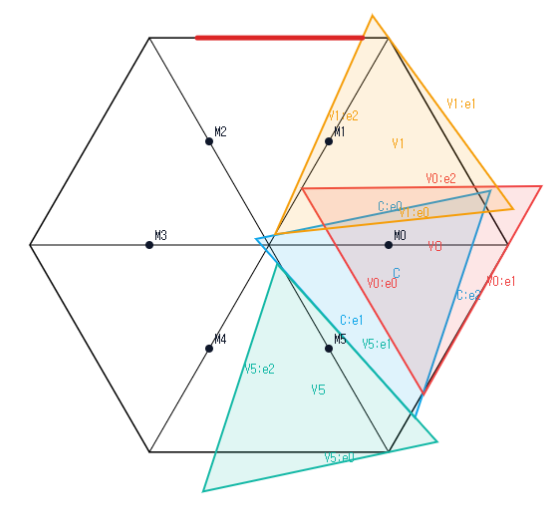
\includegraphics[width=.78\linewidth]
  {figures/strategy2_ce1_ce2_n0_all_vd0.png}
\caption{Schematic view of the common CE1/CE2, $N_+=0$, all-Vd0 boundary
package, not to scale.  The center role and three representative Vd0 vertex
roles are shown; the remaining three roles are omitted for readability.  The
simultaneous placement is not a candidate cover, and no proof depends on
visual inspection.}
\label{fig:ce1-ce2-n0-all-vd0}
\end{figure}

\begin{proposition}[All-Vd0 boundary loss]
\label{prop:nplus-zero-all-vd0}
Assume that $T_C$ is CE1 or CE2, every vertex role is Vd0, and
\[
 A_i+B_i\le1\qquad(0\le i\le5).
\]
Then the seven roles do not cover $H$.
\end{proposition}

\begin{proof}
Let $\mathrm{gr}$ be the number of positive center traces containing an active
V-gap.  Then $\mathrm{gr}\in\{0,1,2\}$, with
$\mathrm{gr}\le1$ in CE1.

If $\mathrm{gr}=0$, the six original open vertex traces cover the connected circle
$\partial H$.  Each has length at most one, and two nonempty members of a
finite relatively open cover must overlap in positive length.  Hence
\[
 6=\Haus(\partial H)
 <\sum_{i=0}^5\Haus(U_i\cap\partial H)
 \le\sum_{i=0}^5(A_i+B_i)\le6,
\]
a contradiction.

Suppose $\mathrm{gr}=1$ and reflect so that the active trace is
\[
 I_R=\left[\frac{k}{R},W+\delta\right].
\]
Put
\[
 s=\frac{k}{R},\qquad q=R-\delta,
 \qquad w_0=W+\delta-\frac{k}{R}.
\]
Then $s+q+w_0=1$.  Gap containment gives $B_0\ge s$ and $A_1\ge q$.
The companion edge has no active gap, so $A_0+B_5\ge1$.  Since row $T_0$ is
nonsupercritical, $A_0+B_0\le1$, and therefore $B_5\ge B_0\ge s$.  The exact
radial demands at the endpoint rows are
\[
 c_1=1-\frac{\delta}{R},
 \qquad
 c_5=1-\frac{\alpha}{W}.
\]
Lemma~\ref{lem:one-side-capped-loss} gives
\[
 F_{c_5}(s)+F_{c_1}(q)<1.
\]
Thus the two actual endpoint outputs satisfy $B_1+B_5<1$.
Lemma~\ref{lem:reader-boundary-path}, applied to $T_2,T_3,T_4$, forces their
total boundary contribution above three, contrary to their three unit caps.

Finally, $\mathrm{gr}=2$ is CE2-only and is exactly
Proposition~\ref{prop:reader-common-two-gap}.  These three ranks are exhaustive.
\end{proof}

We next treat the additional T3-like rows in the $N_+=0$ branch.  The
following local facts also reappear later.

\begin{lemma}[T3-like midpoint and side tradeoff]
\label{lem:t3-midpoint-tradeoff}
Let $T_i$ be T3-like.  Then $M_i\notin T_i$.  After applying the closed-trace
domination of Proposition~\ref{prop:t3-translation}, suppose the selected
adjacent support is on $r_{i+1}$ and $M_{i+1}$ belongs to the dominated
trace.  If $b$ is its boundary reach toward $V_{i+1}$, $c$ its exit on its
own arm, and $\ell$ its entry on $r_{i+1}$, all measured from the relevant
vertex, then
\begin{equation}
 b+c<1,\qquad b+\ell>1.
 \label{eq:t3-side-tradeoff}
\end{equation}
Consequently two adjacent T3-like traces that cover each other's midpoint,
whose selected supports point toward one another, cannot cover both outer
half-arms if no other role has positive support there.
\end{lemma}

\begin{proof}
Apply Proposition~\ref{prop:t3-translation} and reflect if necessary.  Its
translated Type-II majorant has parameters
\[
 0<t<1,\qquad z=\sqrt{1-t+t^2},\qquad \alpha=0,\qquad 0<\beta<z.
\]
Its wedge vertex has
\[
 Q_x=\frac{z-t\beta}{1-t+t^2}>1.
\]
Hence
\[
 t\beta<z-z^2.
\]
The majorant's own-radial exit is $c=\beta/(1-t)$.  Since
\[
 (1-z)(1+z)=t(1-t),
\]
we obtain
\[
 c<\frac{z-z^2}{t(1-t)}=\frac{z}{1+z}<\frac12.
\]
Here $z<1$ because $0<t<1$.  Thus the translated majorant misses $M_0$,
and its closed-trace domination
implies that the original T3-like role misses $M_0$ as well.

For the tradeoff, the translated T3-like trace has the exhaustive Type-II
form
\[
 \begin{aligned}
 (1-t)x+ty&\ge0,\\
 \beta+tx-y&\ge0,\\
 \beta+x-(1-t)y&\le z,
 \end{aligned}
 \qquad 0<t<1,\quad z=\sqrt{1-t+t^2},\quad0<\beta<z.
\]
For the selected support on $r_1$, substitution in the Type-II half-planes
gives
\[
 b=z-\beta,\qquad c=\frac{\beta}{1-t},\qquad
 \ell=\frac{\beta+1-z}{1-t}.
\]
The condition $M_1\in T$ is
$\beta\le z-(1+t)/2$.  Therefore
\[
 b+c\le z+\frac{t}{1-t}
 \left(z-\frac{1+t}{2}\right)
 =1-\frac{(1-z)^2}{2(1-t)}<1,
\]
whereas
\[
 b+\ell-1=\frac{t(1-z+\beta)}{1-t}>0.
\]
For a crossed adjacent pair, coverage forces
$c_i\ge\ell_{i+1}$ and $c_{i+1}\ge\ell_i$.  Combining these two
inequalities with \eqref{eq:t3-side-tradeoff} gives both
$b_i<b_{i+1}$ and $b_{i+1}<b_i$, a contradiction.
\end{proof}

\begin{lemma}[The support-isolated four-label inequality]
\label{lem:407-four-label-loss}
Assume $T_C$ is CE1 or CE2, $N_+=0$, no role is Vd1 or Vd2, and, after
normalization and reflection, $T_0$ is T3-like with selected adjacent
support on $r_1$.  Then the two endpoint rows in the isolated configuration
satisfy
\begin{equation}
 F_{c_5^\ast}(a_5^\ast)+F_{c_1^\ast}(a_1^\ast)<1,
 \label{eq:407-loss}
\end{equation}
where $a_1^\ast,a_5^\ast$ are the exact boundary inputs and
$c_1^\ast,c_5^\ast$ the exact radial demands defined below.
\end{lemma}

\begin{proof}
Use the CE1 side variables $0<\lambda<1$,
$\rho=\sqrt{1-\lambda+\lambda^2}$ and center slacks
\[
 X=F_0(O),\qquad Y=F_2(O).
\]
Then
\[
 a_C=\lambda-Y,\qquad
 \lambda s=X+Y+1-\rho,
\]
and Proposition~\ref{prop:signed-center-normal-form} gives
\[
 \rho-X-Y>\frac12,\qquad
 \frac Y\lambda<\frac12,\qquad
 \frac X{1-\lambda}<\frac12.
\]
Consequently the apparent minima in the two radial exits collapse to
\[
 \gamma_1=\frac Y\lambda,\qquad
 \gamma_5=\frac X{1-\lambda}.
\]
For CE2 the second boundary interval is $[S,T]$, where
\[
 S=\frac{X+Y+1-\rho}{1-\lambda},\qquad T=X+\lambda.
\]

The T3-like normal form supplies $D>1$, $0<R<1$, and $\alpha,p\ge0$ with
\[
 R^2-DR+D^2=1,\qquad \alpha+p=1/D,\qquad
 q=1-p=\alpha+(D-1)/D<1/2.
\]
Its interval on $r_1$, measured from $V_1$, is
\[
 [c,u],\qquad c=Dq/R,\qquad u=q+(1-R)/D.
\]
For an initial trace $[0,p]$ and a center interval $J=[L,U]$, define
\[
 \Theta(p,J)=
 \begin{cases}
 1-p,&J=\varnothing\text{ or }p<L,\\
 1-\max\{p,U\},&p\ge L.
 \end{cases}
\]
Then
\[
 a_1^\ast=\Theta(p,[s,t]),\qquad
 a_5^\ast=\Theta(\alpha,[S,T]),
\]
with the second interval empty in CE1, and
\[
 c_5^\ast=1-\gamma_5,\qquad
 c_1^\ast=
 \begin{cases}
 c,&1-u\le\gamma_1\le1-c,\\
 1-\gamma_1,&\text{otherwise}.
 \end{cases}
\]

If $a_1^\ast+a_5^\ast>1$, the two caps already imply
$F_{c_5^\ast}(a_5^\ast)+F_{c_1^\ast}(a_1^\ast)<1$.  Assume the hard region
$a_1^\ast+a_5^\ast\le1$.  The following table is an exhaustive audit of the four
possible first labels; the middle column records the exact decisive
inequality.
\[
\begin{array}{c|c|c}
\text{first label}&\text{right labels}&\text{conclusion}\\ \hline
L&\mathrm{Full}&e(\gamma_5)<a_1^\ast\\
L&L,T_-&F_{c_5^\ast}(a_5^\ast)+F_{c_1^\ast}(a_1^\ast)<1\\
L&T_+^{\mathrm{hi}}&e(\gamma_5)<a_1^\ast\\
T_-&L,T_-&F_{c_5^\ast}(a_5^\ast)+F_{c_1^\ast}(a_1^\ast)<1\\
T_-&\mathrm{Full},T_+^{\mathrm{hi}}&F_{c_5^\ast}(a_5^\ast)<a_1^\ast\\
\mathrm{Full}&\text{all}&\text{impossible}\\
T_+^{\mathrm{hi}}&\mathrm{Full},T_+^{\mathrm{hi}}&\text{impossible}\\
T_+^{\mathrm{hi}}&L,T_-&F_{c_5^\ast}(a_5^\ast)+F_{c_1^\ast}(a_1^\ast)<1.
\end{array}
\]
We verify the nonformal entries.  Put
$\kappa=(1-\rho)/(1-\lambda)$.  From
$X+(1-\lambda)Y<\rho(1-\rho)$ one obtains
\begin{align}
 \gamma_1\ge a_C&\Longrightarrow e(\gamma_5)<a_C,
 \label{eq:407-core-estimate}\\
 S\le Y/\lambda&\Longrightarrow e(\gamma_5)<S.
 \label{eq:407-S-estimate}
\end{align}
For \eqref{eq:407-core-estimate}, one has
$\gamma_5<a_C-\kappa$ and
$a_C-\kappa<1/8$; then \eqref{eq:low-root-bounds} applies, and the remaining
comparison is
\[
 (a_C-\kappa)+5(a_C-\kappa)^2\le\kappa.
\]
After squaring its positive sides, the difference is
$\lambda(23\lambda^3+58\lambda^2+7\lambda+72)>0$.
For \eqref{eq:407-S-estimate}, combine the premise with the center
inequality and put $x=\lambda$.  This gives $0<x<3/8$ and
\[
 X<X_*=\frac{(1-\rho)(\rho(1-2x)-x(1-x))}{1-x-x^2}.
\]
Set
\[
 \delta=\frac{1-\rho}{1-x}=\frac{x}{1+\rho},\qquad
 \eta=\frac{X}{1-x},\qquad
 f=\rho(1-2x)-x(1-x),\qquad d=1-x-x^2.
\]
Then $\gamma_5\le\eta<\delta f/d$.  Moreover
\[
 \frac fd<1-2x,
\]
because, after multiplication by positive denominators, this is just
\[
 \rho<d+\frac{x(1-x)}{1-2x}
 =1+\frac{2x^3}{1-2x}.
\]
Hence $\eta<\delta(1-2x)<1/8$.  If $\eta=0$, the assertion is immediate.
Otherwise,
\[
 S\ge\frac{X+1-\rho}{1-2x}
 =\frac{1-x}{1-2x}(\eta+\delta)
 >2\eta\left(\frac{1-x}{1-2x}\right)^2.
\]
On the other hand,
\[
 5\eta<5\delta(1-2x)
 <2\left[\left(\frac{1-x}{1-2x}\right)^2-1\right].
\]
For the middle sign use $\rho>1-x$ and
\[
2(2-3x)(2-x)-5(1-2x)^3
 =(4x-3)(10x^2-6x-1)>0
 \qquad(0<x<3/8).
\]
Indeed both factors are negative; for the quadratic use
$10x^2\le15x/4<6x+1$.
The low-root estimate \eqref{eq:low-root-bounds} now gives
\[
 e(\gamma_5)\le2\gamma_5+5\gamma_5^2
 \le2\eta+5\eta^2<S,
\]
proving \eqref{eq:407-S-estimate} without any polynomial coefficient list.
The $L$ separation follows from its exact polynomial: if its output is
$z=e(\eta)$ at input $1-\beta$, then
\[
 \beta\ge z+\eta.
 \label{eq:407-L-separation}
\]
Indeed the selector polynomial
$P(x,z)=x^4-4x^3+5x^2-(2+z)x+z-z^2$ is strictly decreasing on the low
range and vanishes at $x=\eta$.  Equations
\eqref{eq:407-core-estimate}--\eqref{eq:407-L-separation}, with the three
possibilities for $\Theta$, prove every first-$L$ entry.  For a first $T_-$
label the exact root test
\[
 T_-(a,c)<z\iff c^2(a+z)^2-(a^2-ac+c^2)>0
\]
is increasing in $z$.  Substitution of $a_1^\ast$, followed by the center
inequality, proves $F_{c_5^\ast}(a_5^\ast)<a_1^\ast$ except in the low--low entries, which
are immediate from $T_-(a,c)\le\min\{a,1-a\}$ and $L<1/2$.
First-coordinate Full would force either
$X\ge(1-\lambda)\alpha$ and $Y\ge\lambda-\alpha$, contradicting
$s\le p$, or, in the CE2 overlap case, $S\ge1/2$, contradicting
$S\le\alpha<1/2$.

For a first $T_+^{\mathrm{hi}}$ label put $r=1-\lambda$,
$y=Y/\lambda$ and choose $\beta$ so that
\[
 m=\sqrt{\beta^2-\beta+1},\quad
 1-\gamma_5=\frac m{r+\beta},\quad
 F_{c_5^\ast}(a_5^\ast)=\frac{\beta m}{r+\beta}.
\]
The exact selector is
\begin{equation}
 \beta\ge\max\left\{r,\frac12,\frac{1-r^2}{1+2r}\right\},\qquad
 r\ge(1-\beta)(r+\beta)^2.
 \label{eq:407-high-domain}
\end{equation}
The center inequalities give $y<1/10$ and, with
\[
 y_*=\frac r{1-r}
 \left(\frac m{r+\beta}-\frac12-\frac{1-r}{1+\sqrt{r^2-r+1}}\right),
\]
give $y<y_*$ and
\[
 3y_*\le1-\frac{\beta m}{r+\beta}.
\]
This proves the right-$L$ entry by $e(y)<3y$.  It excludes right Full and
right high by the exact high-input filter.  For right $T_-$ with input
$a_C$, direct substitution gives a sum below one.  For input $q$, put
$c=1-y$, $q=tc$, and let $\widehat b_1=F_{c_1^\ast}(q)$.  The selected $T_-$ equations
give
\[
 \widehat b_1\le\kappa:=\frac{\sqrt{13}-1}{6},\qquad
 q\le\tau<\frac{93}{200},
\]
where $\tau\in(0,1/2)$ is the unique root of
$\tau^4-3\tau^3+3\tau^2-3\tau+1=0$.  In this CE2 overlap subcase the
support ordering gives $q>S$.  The common left-high identities are
\[
 S=S_0+\frac{1-r}{r}y,\qquad
 S_0=1-\frac{m}{r+\beta}+\frac{1-r}{1+\sqrt{r^2-r+1}}.
\]
Since $y>0$, we have the complete chain
\[
 S_0<S<q\le\tau<\frac{93}{200}.
\]
We now replace the former interval subdivision by a one-variable comparison.
Write $s=r+\beta$ and $\rho_r=\sqrt{r^2-r+1}$.  The selected Cell~2
inequality factors as
\[
 r-(1-\beta)(r+\beta)^2
 =(s-1)(\beta^2+r\beta-r).
\]
The second factor is nonnegative because $r\le\beta$ and $\beta\ge1/2$;
if it vanishes, then $r=\beta=1/2$.  Hence $s\ge1$.  It follows that
$\rho_r\le m$, since
$\rho_r^2-m^2=(r-\beta)(s-1)\le0$.

Define the one-variable lower bound
\[
 \overline S(\beta)=1-m+\frac{\beta}{1+m}.
\]
Then
\[
 S_0\ge1-\frac m s+\frac{1-r}{1+m}\ge\overline S(\beta).
\]
Indeed, the second difference is
\[
 (s-1)\left(\frac m s-\frac1{1+m}\right)\ge0.
\]
For the last sign use $s\le2\beta\le m(1+m)$: if
$g=3\beta-\beta^2-1$, then $g>0$ and
\[
 m^2-g^2=-\beta(\beta-1)(\beta^2-5\beta+5)\ge0,
 \qquad m^2+g=2\beta.
\]

Put $B_0=5657/10000$, $T=93/200$, and $\beta_*=161/250$.
If $\beta m/s\ge B_0$, then $\beta m\ge B_0$.  The function
$\phi(\beta)=\beta m$ is strictly increasing, and the exact comparison
\[
 B_0^2-\beta_*^2m(\beta_*)^2
 =\frac{22782769}{62500000000}>0
\]
therefore gives $\beta>\beta_*$.  On $[\beta_*,1]$ put
\[
 H(\beta)=\frac{107}{200}-Tm-(1-\beta)^2.
\]
Since $H''=-3T/(4m^3)-2<0$, the function $H$ is concave.  Its endpoint
values are positive: $H(1)=7/100$, while, for
$a_*=107/200-(1-\beta_*)^2=51033/125000$,
\[
 a_*^2-T^2m(\beta_*)^2
 =\frac{1693881}{62500000000}>0.
\]
Thus $H>0$ throughout the interval.  The identity
\[
 (\overline S(\beta)-T)(1+m)=H(\beta)
\]
shows that $\beta m/s\ge B_0$ would force $S_0>T$, a contradiction.
Consequently
\[
 F_{c_5^\ast}(a_5^\ast)<\frac{5657}{10000}
 <\frac{7-\sqrt{13}}6.
\]
The final strict comparison follows by squaring
$\sqrt{13}<18029/5000$, whose squared difference is
$44841/25000000>0$.
Thus the final sum is also below one.  The table is exhaustive, proving
\eqref{eq:407-loss}.
\end{proof}

\begin{proposition}[The $N_+=0$ T3-like branch]
\label{prop:nplus-zero-t3}
Assume that $T_C$ is CE1 or CE2, $N_+=0$, no vertex role is Vd1 or Vd2,
and at least one vertex role is T3-like.  Then the seven roles do not cover
$H$.
\end{proposition}

\begin{proof}
Normalize the unique center midpoint to $M_0$ and simultaneously apply the
closed-trace domination of Proposition~\ref{prop:t3-translation} to every
T3-like role.  If $T_0$ were not T3-like, a maximal consecutive block of
T3-like indices among $1,\ldots,5$ would have to match its roles bijectively
to the same block of uncovered midpoints.  The matching uses only adjacent
indices, because a T3-like role misses its own midpoint and Vd0 roles cannot
cover adjacent midpoints.  Its first two roles therefore form a crossed pair
forbidden by Lemma~\ref{lem:t3-midpoint-tradeoff}.  Hence $T_0$ is T3-like;
reflect so that it supports $r_1$.

There are at most two T3-like roles.  Indeed, with $N_+=0$ and no
Vd1/Vd2 role, the short-role identity gives $q=k$, where $k$ is the number
of T3-like roles.  If $k\ge3$, Theorem~\ref{thm:three-short-roles} gives an
immediate full-skeleton contradiction.
Midpoint locality then forces $T_2,T_4,T_5$ to be Vd0.  Consequently $r_1$
has positive support only from $T_C,T_0,T_1$, and $r_5$ only from $T_C,T_5$.

The actual outgoing reaches of $T_1,T_5$ are bounded by the two safe maps in
Lemma~\ref{lem:407-four-label-loss}; an extra adjacent-ray demand on a
possible T3-like $T_1$ only shrinks its feasible set.  Thus their sum is
less than one.  Rows $T_2,T_3,T_4$ must cover more than three units of the
four intervening boundary edges, while their three nonsupercritical caps
sum to at most three.  This contradiction proves the proposition.
\end{proof}

\begin{lemma}[Free strict-supercritical envelope]
\label{lem:free-supercritical-envelope}
For $0\le c<1/2$,
\[
 \sup\{b:\exists a, (a,b,c)\in\mathcal A, a+b>1\}
 =\mathcal B(c):=\frac{c+\sqrt{c^2-8c+4}}2.
\]
The supremum is not attained.  For $c\ge1/2$ the strict feasible set is
empty.  The function $\mathcal B$ is strictly decreasing on $[0,1/2]$.
\end{lemma}

\begin{proof}
Lemma~\ref{lem:self-midpoint} excludes $c\ge1/2$.  On the boundary
$a=1-b$, a support rotation has strict slack precisely when
\[
 c<\frac{1-b^2}{2-b}.
\]
The right side decreases from $1/2$ to zero.  Solving equality gives the
displayed larger root.  Equality has no strict support slack, which explains
nonattainment.  Differentiation gives
\[
 \mathcal B'(c)=\frac12\left(1+\frac{c-4}{\sqrt{c^2-8c+4}}\right)<0,
\]
since $(4-c)^2-(c^2-8c+4)=12$.
\end{proof}

\subsection{Two reusable capped-loss inequalities}

\begin{lemma}[One-side capped loss]
\label{lem:one-side-capped-loss}
Let $0<R<1$, $S=\sqrt{1-R+R^2}$, and let $s,u,w>0$ satisfy
$s+u+w=1$ and $0<u<R$.  Put
\[
 \delta=\frac{R}{1+S},\qquad
 \gamma=u-\delta-\frac{R}{1-R}w,
\]
and assume $\gamma>0$.  Set
\[
 c_1=u/R,\qquad c_5=1-\gamma.
\]
Then
\begin{equation}
 F_{c_5}(s)+F_{c_1}(u)<1.
 \label{eq:one-side-loss}
\end{equation}
\end{lemma}

\begin{proof}
Put $\eta=(1-R)\delta=1-S$ and
\[
 \widehat b_5=F_{c_5}(s),\qquad
 \widehat b_1=F_{c_1}(u).
\]
The center identity may be written
\begin{equation}
 c_5=\frac{1-u+\eta-Rs}{1-R}.
 \label{eq:one-side-center-line}
\end{equation}
The hypotheses imply $1/2<c_1,c_5<1$: for example
$u>\delta$ gives $c_1>1/(1+S)>1/2$, and
$\gamma<u-\delta<R-\delta=RS/(1+S)<1/2$ gives $c_5>1/2$.
Thus the four high-radial labels of
Proposition~\ref{prop:capped-demand-map} are exhaustive.

\smallskip\noindent
\emph{Right low labels.}
If the right label is $T_-$, its exact frontier equation gives
$(u+\widehat b_1)^2=1-R+R^2=S^2$, so $\widehat b_1=S-u$.  For a right $L$ label write
$\widehat b_1=kc_1$, $0\le k\le1/2$, and $C=1-k+k^2=c_1^2$.  With $X_R=R+k$, the
Cell-$L$ selector factors as
\[
 q=c_1^2(X_R-1)G_k(X_R),\qquad
 G_k(X)=CX^3+CX^2-k(1-k)X+k^2.
\]
For $X\ge k$, $G_k(X)>0$: when $k>0$,
$G_k'(X)\ge k(1+2k-k^2+3k^3)>0$ and
$G_k(k)=k^2(1+k+k^3)>0$.  Hence $q\le0$ gives $X_R\le1$.  If
$h_R=1-X_R$, then
\[
 S^2-(u+\widehat b_1)^2=h_R(1+2k^2+k(1-k)h_R)\ge0.
\]
Consequently either right low label satisfies
\begin{equation}
 \widehat b_1\le X:=S-u.
 \label{eq:one-side-right-low}
\end{equation}

\smallskip\noindent
\emph{A left low label against right high or Full.}
For left $T_-$ put $z=s/c_5=1-p$ and
$h=\sqrt{1-p+p^2}$.  The component selector gives
$0\le p\le1/2$, the frontier gives $s+\widehat b_5=h$, and its selector gives
$s\le(1-p)h$.  Equation \eqref{eq:one-side-center-line} becomes
$c_5(1-Rp)=1-u+\eta$, whence
\[
 u\ge \eta+(1-h)+Rph.
\]
Put $q_0=ph$.  If $q_0>R$, then
$p(1-p)>R(1-R)$ and the preceding lower bound would give $u>R$.
Thus $q_0\le R$, and
\[
 \eta+1-h>
 \frac{R(1-R)+p(1-p)}2\ge(1-R)q_0.
\]
Substitution in the exact formula
\[
 w=\frac{(1-R)(1-u)p-\eta(1-p)}{1-Rp}
\]
now gives $w<1-h$.  A right high output has the form $H-u$, where
$H=\sqrt{1-\beta+\beta^2}\le1$; for Full take $H=1$.  Hence
\[
 \widehat b_5+\widehat b_1=h+H-(s+u)=1+w-(1-h)-(1-H)<1.
\]

For a left $L$ label write
\[
 c_5=h(x):=\sqrt{1-x+x^2},\qquad
 \widehat b_5=xh(x),\qquad 0\le x\le\frac12,
\]
and, along the center line,
\[
 s(x)=\frac{R-u+\eta+(1-R)(1-h(x))}{R}.
\]
If $y=s(x)/h(x)$, the exact selector factorization is
\[
 \frac{q}{h(x)^2}=(y-(1-x))P_x(y),
\]
where
\begin{align*}
 P_x(y)={}&(1-x+x^2)y^3+(1+2x-2x^2+3x^3)y^2\\
 &+(x+2x^2-x^3+3x^4)y+(x^2+x^3+x^5).
\end{align*}
Every coefficient is nonnegative on $0\le x\le1/2$, and the polynomial is
positive at every nondegenerate point.  Thus a selected $L$ point has
$s(x)\le(1-x)h(x)$.  The two curves meet once in $(0,1/2)$: at $x=0$ the
left side is smaller, while at $x=1/2$ it is enough to use
\[
 u\le\frac{R}{1+R}\quad(\mathrm{Full}),\qquad
 u\le\min\{RS,S/2\}\quad(T_+^{\rm hi}).
\]
Writing $e_0=1-\sqrt3/2$, the corresponding endpoint differences are
\[
 \frac{(1-R)(R^2+2Re_0+2e_0)}{2(1+R)}>0
\]
for Full, and respectively
$[2e_0(1-R)-R^3]/2\ge0$ for $R\le1/2$ and
$(1-R)(3R+4e_0-2)/4\ge0$ for $R\ge1/2$ in the high case.
At the unique transition $x_0$, the $L$ frontier is the $q=0$ endpoint of
the preceding $T_-$ branch.  Since $xh(x)$ increases, every selected left
$L$ output is no larger than that transition output.  The preceding strict
loss therefore also covers $(L,T_+^{\rm hi})$ and $(L,\mathrm{Full})$.

\smallskip\noindent
\emph{Full and high exclusions.}
Left Full forces $s<1/2$ and $\gamma\ge s$.  Right Full or right high gives
$u\le1/2$, but
\[
 \gamma-s=2u-1-\delta+\frac{1-2R}{1-R}w<0:
\]
for $R\ge1/2$ this is immediate, while for $R<1/2$ use $w<1-u$ to bound it
by $(u-R)/(1-R)-\delta<0$.  Thus left Full cannot pair with either label.
If the left label is high and the right one Full, then $s<1/2$ and
$u\le R/(1+R)$, whereas $\gamma>0$ and $w>1/2-u$ force
$u>R/2+\eta>R/(1+R)$; the final inequality is equivalent to
$2(1+R)>1+S$.  This pair is also impossible.

\smallskip\noindent
\emph{A right low label.}
Use \eqref{eq:one-side-right-low}.  If $s>X$, the cap gives
$\widehat b_5+\widehat b_1<1$.  Suppose $s\le X$ and put
\[
 c_X=X+2\delta,\qquad f(c,z)=c^4-c^2+zc-z^2.
\]
At the limiting value $u=R$, with $\kappa=\delta$, one has
\[
 X_0=\frac{1-2\kappa}{1+\kappa},\qquad
 c_0=\frac{1+2\kappa^2}{1+\kappa}.
\]
Now $c_0>\sqrt3/2$ because
$16\kappa^4+13\kappa^2-6\kappa+1>0$, and
\[
 f(c_0,X_0)=
 \frac{\kappa^2(1-2\kappa)^2
 (4\kappa^4+4\kappa^3+10\kappa^2+6\kappa+5)}{(1+\kappa)^4}>0.
\]
Along the $u$-line,
$\frac d{du}f(c_X,X)=-4c_X^3+c_X+X<0$, so the same two signs hold before
the limiting endpoint.  Therefore, for
$\ell(c)=c(1-\sqrt{4c^2-3})/2$,
\[
 \ell(c_X)<X<c_X-\ell(c_X),\qquad \ell(c_X)<1-X.
\]

Write $c=h(z)=\sqrt{1-z+z^2}$ and let $z_X$ satisfy $h(z_X)=c_X$.
The actual $c_5(s)$ corresponds to $0<z\le z_X<1/2$, and
\[
 s(z)=s_0+\frac{1-R}{R}(1-h(z)),\qquad
 s_0=\frac{R-u+\eta}{R}>0.
\]
The transition input $(1-z)h(z)$ decreases, and the preceding root ordering
gives $s(z_X)<(1-z_X)h(z_X)$, hence the same strict inequality for all
$z\le z_X$.  To check the order of the two boundary coordinates put
\[
 \phi(z)=s(z)-zh(z),\qquad k_R=\frac{1-R}{R}.
\]
Its endpoint values are $s_0>0$ and $X-\ell(c_X)>0$.  Moreover
\[
 \phi'(z)=\frac{(k_R+z)(1-2z)}{2h(z)}-h(z).
\]
For $k_R\le2$ this is nonpositive; for $k_R>2$ its zero is described by the
strictly increasing function
$K_0(z)=(2-3z+4z^2)/(1-2z)$, so the minimum is again at an endpoint.
Thus $zh(z)<s(z)$.  Applying the already displayed polynomial $P_z$ gives
the strict Cell-$L$ selector, and
$s+zh(z)\le X+\ell(c_X)<1$.  Since
$\partial_bF_L=c(1-2z)>0$ and each feasible fiber is an interval, the capped
maximum is
\[
 \widehat b_5\le zh(z)\le z_Xh(z_X)=\ell(c_X)<1-X.
\]
Together with $\widehat b_1\le X$, this proves the loss for every right low label.

\smallskip\noindent
\emph{High--high.}
Let $c_L(z)$ be the unique root in $[\sqrt3/2,1]$ of $f(c,z)=0$.
With $D_c=4c^3-2c+z>0$, implicit differentiation gives
\[
 c_L''(z)=
 \frac{2(c^2-cz+z^2)+16c^2z(c-z)}{D_c^3}>0.
\]
A selected left high label requires $s<1/2$ and $c_5(s)\le c_L(s)$.
Define
\[
 s_0=\frac{R-u+\eta}{R};
\]
then $0<s_0<s$ and $c_5(s_0)=1$.  The explicitly named function
$g(z)=c_5(z)-c_L(z)$ is concave, with $g(s_0)>0$.  The right high bound
$u\le\min\{RS,S/2\}$ gives $c_5(1/2)>7/8$.  For $R\le1/2$ this follows
after squaring from
$17-10R+9R^2-64R^3-64R^4>0$ (a decreasing polynomial with value $9/4$ at
$1/2$); for $R\ge1/2$ it follows from
$(3+R)^2-16S^2=(1-R)(15R-7)>0$.  Finally
\[
 f(7/8,1/2)=33/4096>0
\]
and $f$ increases in $c$ on this range, so $c_L(1/2)<7/8$ and
$g(1/2)>0$.  Concavity contradicts $g(s)\le0$.  Thus high--high is
impossible.

If both labels are low, the cap already gives
$\widehat b_5+\widehat b_1\le s+u=1-w<1$.  The preceding five paragraphs cover every other
ordered pair of the four labels, proving \eqref{eq:one-side-loss}.
\end{proof}

\begin{lemma}[CE2 two-endpoint capped loss]
\label{lem:two-endpoint-capped-loss}
Let $[x,U]$ and $[y,v]$ be the two exact CE2 traces in the legacy
coordinates of Remark~\ref{rem:signed-legacy-variables}, where $U$ denotes
the endpoint called $u$ there.  Put
\[
 p=1-U,\qquad q=1-v,\qquad
 r=\frac{x}{x+y},\qquad w=\frac{y}{x+y},
\]
and reflect if necessary so that $0<w\le1/2$ and $r=1-w$.  Then
\begin{equation}
 F_{p/w}(p)+F_{q/r}(q)<1.
 \label{eq:two-endpoint-loss}
\end{equation}
\end{lemma}

\begin{proof}
Put
\[
 S_0=x+y,\quad K=\sqrt{1-wr},\quad
 z=\frac{w}{1+K},\quad\zeta=\frac{r}{1+K},
 \quad\alpha=\frac pw,\quad\beta=\frac qr.
\]
Then $D=S_0K$, $1-K=wr/(1+K)$, and the exact midpoint inequalities give
$1/2<\alpha,\beta<1$.  Dividing the coupling equation
$(U+v)S_0-xy=D$ by $S_0$, and using successively $x<U$ and $y<v$, gives
the strict endpoint inequalities
\begin{equation}
 \beta+p>1+z,\qquad \alpha+q>1+\zeta.
 \label{eq:ce2-strict-endpoints}
\end{equation}
Define
\[
 \Phi_w(\alpha)=F_\alpha(w\alpha),\qquad
 \Phi_r(\beta)=F_\beta(r\beta),\qquad
 h(t)=\sqrt{1-t+t^2}.
\]
Thus the desired sum is $\Phi_w(\alpha)+\Phi_r(\beta)$.

\smallskip\noindent
\emph{Selected branch parametrizations.}
For a side of weight $\sigma\in\{w,r\}$, every $L$ label has
\begin{equation}
 c=h(k),\qquad F_c(\sigma c)=kh(k),\qquad0\le k\le w,
 \label{eq:two-endpoint-L-param}
\end{equation}
on either side.  On the large side the range follows from
\[
 Q_{\rm cell}/h(k)^2=(k-w)G_k(r+k),
\]
where
$G_k(X)=h(k)^2X^3+h(k)^2X^2-k(1-k)X+k^2>0$ for $X\ge k$.
The remaining selected parametrizations are
\begin{align}
 \alpha&=\frac{h(a)}{w+a},&
 \Phi_w(\alpha)&=a\alpha,& r\le a<1,
 \label{eq:two-endpoint-small-high}\\
 \beta&=\frac{h(b)}{r+b},&
 \Phi_r(\beta)&=b\beta,& r\le b<1,
 \label{eq:two-endpoint-large-high}\\
 \beta&=\frac K{r+t},&
 \Phi_r(\beta)&=t\beta=K-r\beta,& w\le t\le r.
 \label{eq:two-endpoint-large-tminus}
\end{align}
For example, the small-high selector factors as
\[
 h(a)^2a\left(\frac{w}{(w+a)^2}-(1-a)\right),\qquad
 w-(1-a)(w+a)^2=(a-r)(a^2+wa-w),
\]
which gives $a\ge r$; the other two factorizations are
$(b-w)(b^2+rb-r)$ and $(t-w)(r^2-wt)$, respectively.  These formulas
specify the selected geometric components, not discarded algebraic roots.

The small-side $T_-$ label is absent for $w<1/2$.  Large-side Full is
incompatible with the first inequality in
\eqref{eq:ce2-strict-endpoints}.  Small-side Full can pair only with $L$:
either high or $T_-$ on the large side has $\beta\le K$, which would force
$p>(1+r)z>w/(1+w)$, contrary to Full.  Thus, up to the symmetric
$w=r=1/2$ tie, the exact list is
\begin{equation}
 (\mathrm{Full},L),(T_+^{\rm hi},L),(L,L),(L,T_-),
 (L,T_+^{\rm hi}),(T_+^{\rm hi},T_-),(T_+^{\rm hi},T_+^{\rm hi}).
 \label{eq:two-endpoint-pairs}
\end{equation}

Low--low sums are at most $K<1$: an $L$ output is at most $wK$, while
\eqref{eq:two-endpoint-large-tminus} is at most $rK$.  For Full--$L$, put
\[
 b_{\rm thr}=1+z-\frac{w}{1+w},\qquad
 \kappa=\frac{w}{1+(1+w)z}.
\]
Full and \eqref{eq:ce2-strict-endpoints} give $\beta>b_{\rm thr}$ and
$(1+\kappa)b_{\rm thr}=1+z$.  Direct reduction yields
\[
 b_{\rm thr}^2-h(\kappa)^2
 =\frac{w^2(A(w)+KC(w))}{D_0(w,K)}>0,
\]
where
\begin{align*}
 A(w)&=8-5w+22w^2+6w^3+5w^4+5w^5-w^6,\\
 C(w)&=8-w+14w^2+4w^3-2w^4+w^5,\\
 D_0(w,K)&=((1+w)(1+K))^2(1+K+w+w^2)^2.
\end{align*}
Both numerator polynomials are positive on $[0,1/2]$.  Since $h$ decreases
and $(1+k)h(k)$ increases there,
$\beta=h(k)>b_{\rm thr}>h(\kappa)$ implies
$(1+k)\beta<1+z$; combined with \eqref{eq:ce2-strict-endpoints}, this gives
$k\beta<p$ and hence the strict Full--$L$ loss.

It remains to verify the four pairs containing a high label on the small
side.

\smallskip\noindent
\emph{$(L,T_+^{\rm hi})$.}
Use parameters $0\le k\le w$ and $r\le t<1$:
\[
 \alpha=h(k),\quad\Phi_w=kh(k),\qquad
 \beta=\frac{h(t)}{r+t},\quad\Phi_r=\frac{th(t)}{r+t}.
\]
The first output and the last output increase in their parameters, while
$h(t)/(r+t)$ decreases.  If $w\le2/5$, then
\[
 \Phi_w+\Phi_r<wK+\frac1{2-w}<1;
\]
after using $K\le1-wr/2$, the positive cleared gap is
$P(w)=w^4-3w^3+4w^2-6w+2$, which decreases on $[0,2/5]$ and has
$P(2/5)=46/625$.  If $w\ge2/5$, the first endpoint inequality gives
$\beta>r+z\ge3/4$.  Since
$h(3/4)/(r+3/4)=\sqrt{13}/(7-4w)<3/4$, monotonicity forces $t<3/4$.
Therefore
\[
 \Phi_w+\Phi_r<\frac{\sqrt3}{4}+\frac{3\sqrt{13}}{20}<1.
\]

\smallskip\noindent
\emph{$(T_+^{\rm hi},T_-)$.}
Use $a,t$ from \eqref{eq:two-endpoint-small-high} and
\eqref{eq:two-endpoint-large-tminus}.  Both demands are at most $K$.
The first endpoint inequality gives
\[
 \alpha>\frac{1+z-K}{w}=\frac{1+r}{1+K}=:a_0.
\]
Thus $K>1-w^2$, which forces $w>1/3$, and comparison at $a=2/3$ forces
$a<2/3$.  The function
\[
 G(a)=\frac{(1+a)h(a)}{w+a}
\]
decreases on $[r,2/3]$, because its derivative numerator
$2a^3+(4w-1)a^2+(1-w)a+w-2$ is at most its value
$-7/54$ at $(2/3,1/2)$.  Hence $G(a)\le(1+r)K$.
Using the second endpoint inequality and
$\Phi_r=K-r\beta$ gives
\[
 \Phi_w+\Phi_r<(2+r)K-1-\zeta<1.
\]
After multiplication by $1+K$, the last positive gap is
$r(3w-w^2-K)$; its squared comparison is
\[
 (3w-w^2)^2-K^2=w^4-6w^3+8w^2+w-1>0
\]
for $w>1/3$ (value $1/81$ at $1/3$, positive derivative thereafter).

\smallskip\noindent
\emph{$(T_+^{\rm hi},T_+^{\rm hi})$.}
Use parameters $a,b$ from \eqref{eq:two-endpoint-small-high}--
\eqref{eq:two-endpoint-large-high}.  The endpoint inequalities first force
$w>2/5$: for $w\le2/5$, the asserted contrary inequality
$K(w+1/(2r))\le1+z$ reduces, after multiplication by $2r(1+K)$, to
\[
 K(2w^2-4w+1)+2w^4-4w^3+w^2-w+1>0,
\]
which is immediate according as the coefficient of $K$ is nonnegative or,
using $K\le1$, from the decreasing polynomial
$2w^4-4w^3+3w^2-5w+2\ge172/625$.

For $F_c(t)=(1+t)h(t)/(c+t)$, the derivative numerator
$2t^3+(4c-1)t^2+(1-c)t+c-2$ is increasing on the present rectangle, so
$F_c$ has at most one interior minimum.  Endpoint comparison gives
\[
 \Phi_w+\alpha\le\frac2{1+w},\qquad
 \Phi_r+\beta\le\frac2{1+r}.
\]
The nontrivial endpoint signs are exactly
\[
 4-(1+r)^2(1+w)^2K^2
 =-w^2(w-1)^2(w^2-w-3)>0
\]
and
\[
 16r^2-(1+r)^4h(r)^2
 =(1-r)(r^5+4r^4+7r^3+9r^2-4r-1)>0;
\]
the bracket is increasing on $[1/2,1]$ and equals $13/32$ at $1/2$.
Weighting the two strict endpoint inequalities by $w/K^2$ and $r/K^2$
gives
\[
 \alpha+\beta>\frac{2K+1}{K(1+K)}.
\]
Consequently
\[
 \Phi_w+\Phi_r<\frac2{1+w}+\frac2{1+r}
 -\frac{2K+1}{K(1+K)}<1.
\]
The numerator of the last gap is $3Kwr-Q(w)$, where
$Q(w)=w^4-2w^3+7w^2-6w+2>0$.  Its squared difference is
\[
 D(w)=-w^8+4w^7-9w^6+13w^5-41w^4+65w^3-55w^2+24w-4.
\]
Here $D'(w)=(1-2w)H(w)$ with
\[
 H(w)=4w^6-12w^5+21w^4-22w^3+71w^2-62w+24>0
\]
on $[2/5,1/2]$; use
$71w^2-62w+24\ge743/71$ and the remaining cubic block at least $-11/4$.
Thus $D$ increases and $D(2/5)=4904/390625>0$, proving the claim.

\smallskip\noindent
\emph{$(T_+^{\rm hi},L)$.}
Use the fully specified parameters
\[
 \alpha=\frac{h(t)}{w+t},\quad p=w\alpha,\quad b=t\alpha,
 \quad\frac12\le t<1,
\]
and
\[
 \beta=H=h(k),\quad \widehat b_L=kH,\quad 0\le k\le w.
\]
Since $p+b=h(t)$, the first endpoint inequality gives
\begin{equation}
 1-(b+kH)>G:=2+z-h(t)-(1+k)H.
 \label{eq:two-endpoint-high-L-G}
\end{equation}
Put
\[
 p_0=1+z-K=\frac{w(2-w)}{1+K},
\]
let $t_0\in(1/2,1)$ be the unique point with
$p(t_0)=wh(t_0)/(w+t_0)=p_0$, and put $b_0=t_0p_0/w$.
The exact endpoint lemma is
\begin{equation}
 b_0<1-wK.
 \label{eq:two-endpoint-b0}
\end{equation}
To verify it, set $b_*=1-wK$ and $T_*=wb_*/p_0$.  One has $0<T_*<1$, and
\[
 p_0^2(w+T_*)^2-w^2h(T_*)^2
 =-\frac{w^3(KE(w)+J(w))}{(1+K)^2(2-w)^2}>0,
\]
where
\[
 E(w)=2w^5+3w^3-20w^2+23w-6,
\]
\[
 J(w)=w^6+8w^5-22w^4+12w^3+6w^2+2w-6.
\]
Here $J\le-111/64$; if $E>0$, then
$KE+J<E+J<0$, because $E+J$ is increasing and equals $-139/64$ at
$w=1/2$.  Thus $p(T_*)<p(t_0)$.  Since $p(t)$ decreases,
$t_0<T_*$ and \eqref{eq:two-endpoint-b0} follows.

Finally put $P=1+z-p$.  If $P<K$, then $t<t_0$ and $k\le w$, so
\[
 G>2+z-h(t_0)-(1+w)K=1-b_0-wK>0.
\]
If $P\ge K$, then $K\le P\le P_1:=1+z-w/(1+w)\le1$ and there is
$a\in[0,w]$ with $h(a)=P$.  Since $P<H$, one has $k<a$ and
$(1+k)H<(1+a)P=P+\ell(P)$, where
$\ell(P)=P(1-\sqrt{4P^2-3})/2$.  Hence
\[
 G>\mathcal D(P):=1-b(P)-\ell(P).
\]
This function is concave.  Indeed $\ell''(P)>0$, and the high output $b$ is
convex in $p=1+z-P$: with
$A_t=2+w-(1+2w)t>0$ and
$Q_t=8wt^2+4t^2-8wt-13t-w+4<0$,
\[
 \frac{d^2b}{dp^2}=-\frac{2h(t)(t+w)^3Q_t}{w^2A_t^3}>0.
\]
At $P=K$, \eqref{eq:two-endpoint-b0} gives
$\mathcal D(K)=1-b_0-wK>0$.  At $P=P_1$, set
$\kappa=w/(1+(1+w)z)$.  The Full--$L$ comparison already proved gives
$P_1>h(\kappa)$, hence
$\ell(P_1)<\kappa P_1=w/(1+w)$, while $b(P_1)=1/(1+w)$.
Thus $\mathcal D(P_1)>0$, and concavity gives $G>0$ throughout.
Equation \eqref{eq:two-endpoint-high-L-G} proves the final hard pair.

The exact list \eqref{eq:two-endpoint-pairs} is now exhausted, proving
\eqref{eq:two-endpoint-loss}.
\end{proof}

\subsection{The exactly-one-Vd1/Vd2 placements}

We now assume CE2, $N_+=1$, and exactly one row is Vd1 or Vd2.  The corner
normal form of Proposition~\ref{prop:vd-corner-normal-form} will be used in
the following form: for some $t>0$ and $d=\sqrt{t^2+t+1}$,
\begin{equation}
 x-(t+1)y\le a,\qquad ty-(t+1)x\le tb,\qquad
 tx+y\le d-a-tb.
 \label{eq:vd-corner-form}
\end{equation}
In particular $a+b<1/2$ for a positive-support row.

\begin{lemma}[Vd1 adjacent rescue]
\label{lem:vd1-adjacent-rescue}
Assume an original open-role skeleton cover in the CE2 exact-$M_0$ branch,
with $T_0$ the unique Vd1 row, $M_1\in T_0$, $T_1$ uniquely supercritical,
$T_2,\ldots,T_5$ nonsupercritical Vd0, and no other positive-adjacent-support
role.  Then the perimeter together with $r_1$ is not covered.
\end{lemma}

\begin{proof}
Lemma~\ref{lem:short-vd1-rescuer-profile} proves the two local inequalities
in \eqref{eq:signed-rescuer-local}.  Midpoint and support isolation force the
center to cover the $O$-side radial gap before the Vd1 interval.  The result is
therefore Corollary~\ref{cor:signed-adjacent-rescuers}.
\end{proof}

\begin{lemma}[Vd1--supercritical replacement]
\label{lem:vd1-pair-replacement}
\leavevmode\par\noindent
Assume an original open-role perimeter-and-radial-skeleton cover in the CE2
exact-$M_0$ branch and the complementary no-additional-positive-support
case.  Let $T_i$, $i\ne0$, be uniquely supercritical, and let the unique Vd1
row, distinct from $T_0$ and adjacent to $T_i$, contain $M_i$.  Assume every
other vertex row is nonsupercritical Vd0 and the center has no boundary trace
on the shared edge of this pair.  Then the pair can be replaced by two open
nonsupercritical Vd0 roles preserving all boundary and radial demands used
by Proposition~\ref{prop:nplus-zero-all-vd0}.
\end{lemma}

\begin{proof}
Normalize the Vd1 row at $V_0$ and the supercritical row at $V_1$.
By the shared-edge hypothesis, no center trace intervenes on $e_{0,1}$;
by the no-additional-positive-support hypothesis, no third vertex role has
positive boundary or radial support in the handoffs used below.
In \eqref{eq:vd-corner-form}, midpoint rescue and one-sided support imply
$t\ge1$ and, with
\[
 c=\frac{d-a-tb}{t+1},\quad
 \lambda=\frac{t(1-b)}{t+1},\quad
 \mu=\frac{d-a-tb-1}{t},
\]
give the strict consequences
\begin{equation}
 a+c<1,\qquad a<\lambda\le\frac12,\qquad
 b<\frac12,\qquad \mu<1-a.
 \label{eq:replacement-margins}
\end{equation}
The shared edge forces the supercritical input $A_i\ge1-b>1/2$, and radial
coverage forces $C_i\ge\lambda$.  A direct consequence of
Proposition~\ref{prop:exact-admissible-set} is
\[
 (x,y,z)\in\mathcal A,\quad x\ge1/2,\quad z\le1/2
 \quad\Longrightarrow\quad y\le1-z.
\]
Indeed, substituting $x=1/2,y=1-z$ in the selected supercritical polynomial
gives $z^2(2z-5)(2z-1)/4\ge0$, and the polynomial is increasing in both
relevant coordinates.  Hence $B_i\le1-C_i\le1-\lambda$ and
$a+B_i<1$.  Open radial handoff further gives
\[
 c_i^{\rm req}<\max\{C_i,\mu\}
 \le\max\{1-B_i,1-a\}.
\]

Choose $p_1,p_2$ within these margins so that
\[
 a<p_1<p_2<1-B_i,\qquad
 p_1<\frac12,\qquad
 1-p_1>c,\qquad
 \max\{p_2,1-p_2\}>c_i^{\rm req}.
\]
In local coordinates define the closed unit-triangle templates
\[
 \Delta_p^-=\conv\{(0,1-p),(1,1-p),(0,-p)\},
 \quad 0\le p\le1/2,
\]
and
\[
 \Delta_p^+=\conv\{(p,0),(p,1),(p-1,0)\},
 \quad 1/2<p\le1.
\]
Their incident reaches are $p,1-p$, their own-radial reach is respectively
$1-p,p$, and they have zero adjacent support.  Define
\[
 X_{\rm loc}:\mathbb R^2\to\mathbb R^2,\qquad
 X_{\rm loc}(x,y):=V_0+x(V_5-V_0)+y(V_1-V_0).
\]
Choose
\[
 0<\varepsilon<
 \min\{p_1-a, p_2-p_1, 1-B_i-p_2,
 1-p_1-c, \max\{p_2,1-p_2\}-c_i^{\rm req}\}
\]
and set
\[
 T_0':=
 X_{\rm loc}\!\left(\interior(\Delta_{p_1}^-)+(-\varepsilon,0)\right),
\]
\[
 T_1':=
 \begin{cases}
 X_{\rm loc}\!\left(\interior(\Delta_{p_2}^-)
 +(-\varepsilon,0)\right),&p_2\le1/2,\\
 X_{\rm loc}\!\left(\interior(\Delta_{p_2}^+)
 +(0,-\varepsilon)\right),&p_2>1/2.
 \end{cases}
\]
The closures of $T_0'$ and $T_1'$ have the same supremal reaches as the
translated templates.  Thus the two replacements are open Vd0 roles with
boundary sum $<1$, while the chosen strict margins preserve the shared
boundary and both radial handoffs.  The datum therefore reduces to
Proposition~\ref{prop:nplus-zero-all-vd0}.
\end{proof}

\subsection{Exact-demand terminal routing}

\begin{proposition}[Exact-demand terminal branches]
\label{prop:demand-branches}
The exact-demand method proves the following terminal exclusions:
\begin{enumerate}
\item CE1 or CE2, $N_+=0$, all vertex roles Vd0;
\item CE1 or CE2, $N_+=0$, with at least one T3-like role and no Vd1/Vd2;
\item CE1 or CE2, $N_+=1$, all vertex roles Vd0, with at least one boundary
gap;
\item CE1 or CE2, $N_+=1$, exactly one T3-like role and no Vd1/Vd2;
\item the CE2, $N_+=1$, exactly-one-Vd1/Vd2 branch.
\end{enumerate}
All gap alternatives include singleton gaps.
\end{proposition}

\begin{proof}
The five items are respectively Propositions
\ref{prop:nplus-zero-all-vd0}, \ref{prop:nplus-zero-t3},
\ref{prop:nplus-one-all-vd0}, \ref{prop:nplus-one-one-t3}, and
\ref{prop:signed-ce2-one-vd-placements}.  The strictness at open handoffs appears in
the weak endpoint bounds, the nonattained supercritical envelope, and the
strict replacement margins; no positive-length assumption is made about a
V-gap itself.
\end{proof}
